% Writeup for MDS
% David Lawrence Miller
% d.l.miller@bath.ac.uk
  
\documentclass[a4paper,10pt]{article}
\setlength{\textheight}{22.5cm}
\setlength{\textwidth}{6.47in}
\setlength{\oddsidemargin}{-1mm}
\setlength{\topmargin}{0.1cm}
\setlength{\evensidemargin}{-5mm} 
 
% Load some packages
\usepackage{times, amsmath, amssymb, amsfonts, url, natbib, bm, rotating}
 
\usepackage{multirow}
\usepackage{graphicx}
\usepackage{rotating}

% top matter
\title{Multidimensional scaling as a tool for \\smoothing over complex regions}
\author{David Lawrence Miller\\Mathematical Sciences\\University of Bath\\\texttt{d.l.miller@bath.ac.uk}}
 
% Shortcuts
% Probability
\newcommand{\prob}[1]{\mathbb{P}\left[ #1 \right]}
% Schwarz-Christoffel
\newcommand{\sch}{Schwarz-Christoffel }
% fprime
\newcommand{\fprime}{f^\prime(z)}
% figure reference command
\newcommand{\fig}[1]{\emph{fig.} \ref{#1}}
% Figure reference command
\newcommand{\Fig}[1]{\emph{Fig.} \ref{#1}}
% table reference command
\newcommand{\tabref}[1]{\emph{table} \ref{#1}}
% Table reference command
\newcommand{\Tabref}[1]{\emph{Table} \ref{#1}}
% equation reference command
\newcommand{\eqn}[1]{(\ref{#1})}
% phi inverse
\newcommand{\phiinv}{\phi^{-1}}
% use other phi
\renewcommand{\phi}{\varphi}
%transpose
\newcommand{\tr}[1]{#1^{\text{T}}}
% diagonal
\newcommand{\diag}{\text{diag}}
% call \times \cross
\newcommand{\cross}{\times}


\begin{document}
 
% The abstract
%\begin{abstract}
%Here.
%\end{abstract}
 
 
% New theorem for theorems
\newtheorem{thm}{Theorem}[section]
 
%New theorem for definitions
\newtheorem{defn}{Definition}[section]
 
\maketitle

\section{Introduction}

\subsection{Motivation}

Splines are a popular way of performing spatial smoothing in two dimensions. In this context, they are used to fit smooth functions over a geographical region. A typical application of this is in ecological modelling; particularly when the spatial distribution of a species is sought. In this case counts of the species in question at the locations at which they were observed are recorded and fed into the model which can then be used to perform inference on the population, whether that be an abundance estimate, density map or a more sophisticated inferential goal.

When the geographical region has a complex boundary, features from one part of the domain can unduly influence other parts. Typically a ``complex boundary'' consists of having some peninsula-like feature(s) in the domain with notably different values on either side of the feature; there must also be some scientific motivation as to why those parts of the domain should not affect each other. Features such as peninsulae give rise to a phenomenon known as leakage; a typical example can be seen in \fig{leakage}. Leakage is problematic since it causes the fitted surface to be mis-estimated; this can then lead to incorrect inference (eg. incorrect abundance estimates), which is clearly not desirable. This can be seen in \fig{leakage} where the high values in the upper part of the domain leak across the gap to the lower values below and vice versa.

The cause of leakage can be thought of in two ways: either the smooth does not respect the boundary of the domain, or the smooth does not take into account the internal geometry of the domain; in particular with regard to the distance between points in the domain. Previous work in this area has been to combat leakage along these two lines. Work of \cite{ramsay} and \cite{soap} both use a PDE boundary condition approach to try to prevent leakage, where as \cite{wangranalli} attempt to approximate the within-area distances. In this report I will be adopting the the latter approach.

% leakage example 
\begin{figure}
\centering
% trim order l b r t
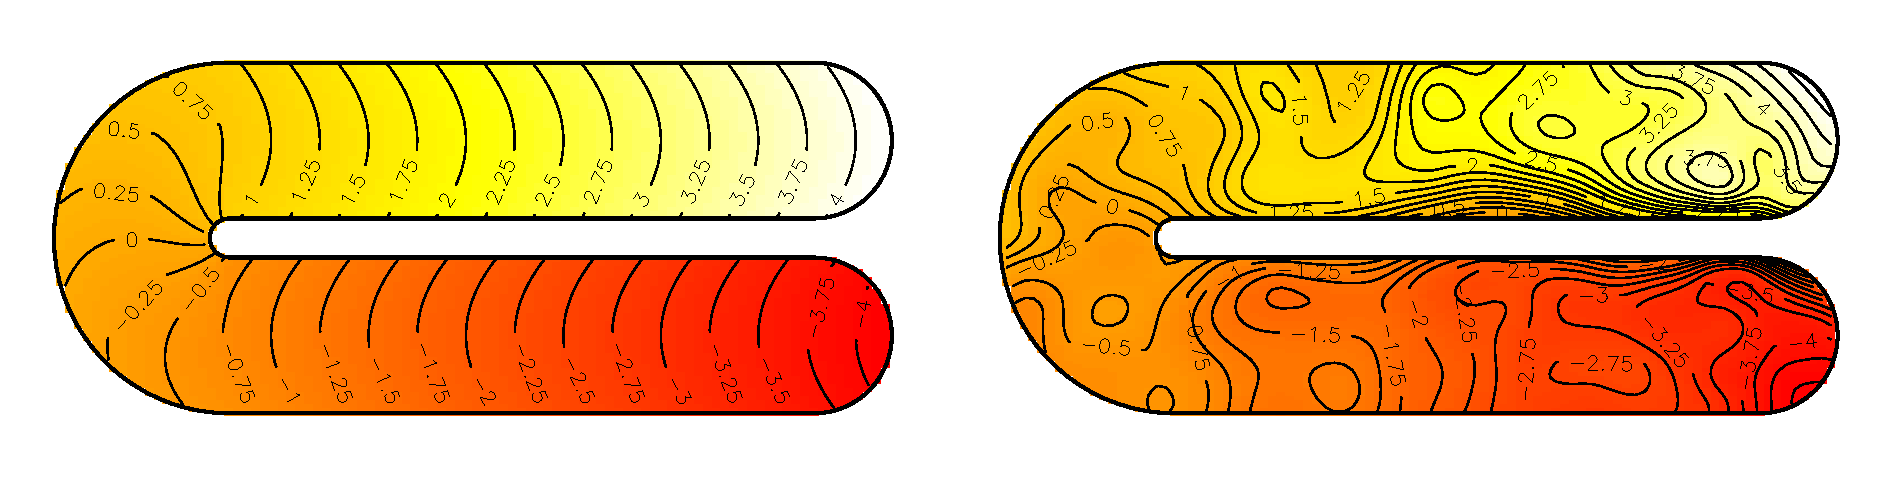
\includegraphics[width=4in]{figs/ramsay-leak.pdf}\\
\caption{An example of leakage. A thin plate regression spline was fit to data sampled from the function on the left, here the model smooths across the gap in the middle of the domain (right.)}
\label{leakage}
\end{figure}


\subsection{Proposition}

Multidimensional scaling (MDS) or, as it is often referred to, principle coordinates (PCO) (\cite{gower1966}) is a method commonly used in multivariate analysis. It is closely related to techniques such as PCA (\cite{chatfieldcollins}, p. 200) and canonical correspondence analysis (\cite{terbraak}.) The starting point for MDS is a matrix of distances, representing some kind of dissimilarity between observations. This distance could be calculated from the data, for example ideological distance between politicians measured using NOMINATE scores (\cite{quantss}, p. 225), or could instead be distances that occur in the data naturally,  for example comparative distances between stimuli response in a psychological experiment (\cite{torgerson}.) Here we concentrate on geographical distances.

MDS takes this matrix of distances and projects the data in such a way that Euclidean inter-point distances in the projection are approximately the same as the distances in the matrix (\cite{chatfieldcollins}, p. 187.) If the matrix of distances is of rank $m$ then a projection in $m-1$ or less can be output, although a projection into 2 dimensions is a typical choice. For this reason one can also think of MDS as a dimension reduction technique, finding a projection of a data cloud into lower dimensional space, while still retaining information about the distances between the points.

When MDS is performed on some categorised set of dissimilarities (as is often the case in social science and psychology) it is referred to as non-metric MDS, where as on a continuous scale it is known as metric MDS, though they have different names, the calculations are identical (aside from the method of finding the distances.) Discussion here will focus on metric MDS.

Multidimensional scaling offers a framework for the problem of smoothing over a region with a complex boundary. Given the set of distances between the points in the domain, we can project those points into a configuration such that the distances between those points are approximately preserved. Now, if the Euclidean metric were to be used to calculate the distances between the points then the result from the projection would be identical to the starting point configuration (provided that we projected back into the same number of dimensions.) However, if it were possible to use a metric that took into account the distance within the boundary (a within-area distance) then the resulting configuration of points would (approximately) respect the boundary of the domain.

This approach can be justified in the following way. In many applications within-area distances is meaningful, given (as stated above) that there is some reasoning behind why certain parts of the domain should not affect one another. When within-area distances are meaningful, it makes sense to work with the structure of the domain rather than the somewhat arbitrary choice of Euclidean geometry. However, as literature on smoothing is firmly based in a Euclidean context, it would be preferable to perform the smoothing in Euclidean space. In this case the approximation to Euclidean space afforded by an MDS projection of the within-area distances offers a bridge between these two requirements.

\subsection{Procedure}

The proposed procedure is as follows: Given a sample $\{x_i, z_i : i=1\dots n\}$: the set of points in the domain over which smoothing is to be performed, $x_i$ is the location (a $k$-vector, although here 2-vectors are assumed throughout) of the $i^\text{th}$ point with response $z_i$. Here it is assumed that finding an MDS configuration of a set of points includes calculating the within-area distances between the points and then the distance matrix, as well as actually performing the MDS calculation.

\begin{enumerate}
\item Obtain the MDS configuration for the domain using some representative set of points over the area in question. The only use of the MDS locations obtained in this step is to define the configuration, they are discarded afterward. Representative points could be a grid over the domain or subset of $\{x_i : i=1\dots n\}$; more detail and justification is provided in section \ref{grids}, below.

\item Using the MDS configuration obtained above along with Gower's interpolation (see section \ref{gowers}) obtain the location of the sample in the MDS configuration: $\{\tilde{x}_i, z_i : i=1\dots n\}$.

\item Smooth $\{\tilde{x}_i, z_i : i=1\dots n\}$ using a regression spline.

\item To predict at a location $x_j$ in the original domain, use Gower's interpolation to 
obtain the point's location in the MDS space: $\tilde{x}_j$. Predict $\hat{z}_j$ using the smooth at $\tilde{x}_j$: this is the prediction at $x_j$.
\end{enumerate}

The rest of this report is structured as follows: in section 2 an overview of MDS is given, along with technical details of how the MDS configuration is calculated; section 3 focuses on how the within-area distances are found; section 4 shows some examples of this method on simulated data. I conclude with a proposed course of action to improve the method.

\section{Multidimensional Scaling}

The basic concept behind MDS is to take the data, calculate their within-area inter-point distances and then find a new coordinate system based on those inter-point distances. We do this by simply performing an eigen-decomposition on the (centred) matrix of distances between points. First a description of the MDS procedure when Euclidean distances are used is given, followed by the justification for the use of the same procedure when using within-area distances.

\subsection{Finding the new point configuration}

We first define $d_{ij}$ as the distance between the points $i$ and $j$. These are used to form a (symmetric) matrix, $D$, with $ij^{\text{th}}$ element $d^2_{ij}$. For the moment let us assume that $D$ is known and $d_{ij}$ Euclidean distance between points $i$ and $j$. 

\cite{diaconis08} gives a clear definition of the algorithm (due to \cite{schoenberg35} and \cite{torgerson}) for finding the new locations of points, which is outlined below. Further detail is given in \cite{principlesofMA}, pp. 104-108 and \cite{chatfieldcollins}, pp. 189-200.

First, suppose that the $n$ the unknown locations (in $n$ dimensions) in our MDS configuration are entries in an $n \times n$ matrix, $\tilde{X}^*$. Now let $S=\tilde{X}^{*} \tilde{X}^{*\text{T}} $, so $S$ is a matrix of scalar products of the point vectors, \emph{ie.} the $(i,j)^\text{th}$ element of $S$ is:
\begin{equation}
s_{ij} = x_i\tr{x_j},
\label{selem}
\end{equation}
$S$ is an $(n\cross n)$ matrix. Note that we may only find $\tilde{X}^*$ up to a translation and rotation, so it is assumed that the values in $\tilde{X}^*$ have been centred about the origin.

We now wish to relate $D$ to $S$. First, note that that $(i,j)^\text{th}$ element of D is 
\begin{equation}
d_{ij}^2 = (x_i-x_j)\tr{(x_i-x_j)} = x_i\tr{x_i} + x_j\tr{x_j}  -2 x_i\tr{x_j}.
\label{dij}
\end{equation}
Using \eqn{selem}, we can re-write \eqn{dij} as
\begin{equation}
D=\mathbf{s}_\text{diag}\tr{\mathbf{1}} + \mathbf{1}\tr{\mathbf{s}_\text{diag}} -2S.
\label{dijmat}
\end{equation}
where $\mathbf{1}$ is an $n \cross 1$ vector of 1s and $s_\text{diag}$ is the $n \cross 1$ vector of diagonal elements of $S$.

Defining:
\begin{equation}
H = I-\frac{1}{n}\mathbf{1}\tr{\mathbf{1}},
\end{equation}
where $I$ is the identity matrix, as usual, and $\mathbf{1}$ is an $n \cross 1$ vector of 1s such that $\mathbf{1}\tr{\mathbf{1}}$ is an $n \cross n$ matrix of 1s.

By pre- and post-multiplying any matrix by $H$ the matrix is double centred (such that row and column means are 0.) This is true since, pre- and post-multiplying \eqn{dijmat} by $H$ yields:
\begin{equation}
HDH = -2HSH.
\label{eqH}
\end{equation}
The first two terms in on the right hand side of \eqn{dijmat} going to zero since the rows of $\mathbf{s}_\text{diag}\tr{\mathbf{1}}$ and the columns of  $\mathbf{1}\tr{\mathbf{s}_\text{diag}}$ are constant. Since $S$ is already centred, $HSH=S$, so the following relation between $S$ and $D$ holds:
\begin{equation}
S = -\frac{1}{2}HDH.
\label{eqH}
\end{equation}

Now we can deal with $S$ rather than $D$. We must factor $S$ find $\tilde{X}^{*}$. One option to factor $S$ is to use the Cholesky decomposition, however, with MDS we are looking to decompose the space based on the directions of largest variation, \emph{ie.} those that have the largest contribution to $s_{ij}$. For that reason we use the eigen-decomposition.

Performing an eigen-decomposition n $S$, we obtain $S=U\Lambda\tr{U}$. Here $U$ is the $n \cross n$ orthogonal matrix of eigenvectors and $\Lambda$ is the $n \cross n$ diagonal matrix of eigenvalues, we may then obtain $\tilde{X}^*$ as:
\begin{equation}
\tilde{X}^*=U\Lambda^{\frac{1}{2}}.
\end{equation}

Following these steps $\tilde{X}^*$ is an $n \cross n$ matrix. The aim here is to smooth in two dimensions (and in general we would preform MDS and want to see a reduction in dimensionality) so, the directions with the two largest eigenvalues are chosen to represent the space since they contain the two largest sources in variation in distance (since they are the two largest contributions to $S$.) This gives the two dimensional representation of the data. So, defining $\tilde{X}$ to be the $n \cross 2$ dimensional matrix obtained from truncating the full new coordinate set to the first two columns in decreasing eigenvalue order, a lower dimensional representation has been obtained. More generally, we can reduce the $\tilde{X}^*$ to an $n \cross k$ matrix, where $k$ is the number of dimensions for the MDS representation of the data.

So, in order to obtain the MDS configuration of points (given that we have some set of inter-point distances) we merely need to double centre the matrix of distances and perform an eigen-decomposition on the resulting matrix, $S$. 

In our case, we would like $d_{ij}$ to be the shortest distance between the points, given the path between the points remains within the domain. Finding $d_{ij}$ is discussed in the next section, however it is first important to justify the use of these steps when non-Euclidean distances are used. 

One can think of the justification in the following way: given that the distances in $D$ obey the triangle inequality, all of the points in $D$ ($n$ of them if $D$ is $n \cross n$) may be represented in $n$ dimensional Euclidean space (at worst.) Hence, in the case where the $d_{ij}$ are Euclidean distances in two dimensions, the smallest dimensional space in which they can be represented is 2, but they may still reside in $n$-dimensional space with no loss of information about the distances. So, in the case when the distances in $D$ are shortest within-area distances, one can just think of the points in $D$ as residing in a higher number of dimensions in such a way that the distances between them are Euclidean.

Note that an additive constant can be computed and added to the non-diagonal entries of $D$ to ensure that the eigenvalues of $S$ are non-negative. However, this does not occur in any of the examples shown here.

Multidimensional scaling may be performed in \textsf{R} using the \texttt{cmdscale} function. 

\subsection{Gower's interpolation} 
\label{gowers}
It is likely that we may be in a position where the coordinate system has been found by MDS but we need to insert further points into our MDS representation for example when further data is collected, or in order to predict over points not in $\tilde{X}$. In this case we would like to insert those new points into the configuration given by MDS. A number of methods have been developed over the past 40 years; Gower's interpolation (\cite{gower1968}) is covered here.

Say we have some point, $x_{\text{new}}$ and we wish to find its new location, $\tilde{x}_{\text{new}}$ in the MDS configuration, $\tilde{X}$. The position of $\tilde{x}_{\text{new}}$ is at a distance from the points in $\tilde{X}$ which is approximately the same as that of $x_{\text{new}}$ to the points in the non-transformed space. 

Note that here we are assuming that a 2 dimensional projection has been used in the initial MDS configuration, obviously Gower's interpolation remains valid for the case in which the initial MDS projection is in $k$ dimensions.

\subsubsection{Gower's interpolation formula}

We may find the new position, $\tilde{x}_{\text{new}}$ , of some new datum $x_{\text{new}}$ using:
\begin{equation}
\tilde{x}_{\text{new}} = \frac{1}{2} \Lambda^{-1} \tr{\tilde{X}} \mathbb{D}.
\label{gower}
\end{equation}
Here $\Lambda$ ($2 \cross 2$) and $\tr{\tilde{X}}$ ($2 \cross n$) are as above, $\mathbb{D}$ ($n \cross 1$) is the centred distance from the points in the original configuration to the new point.

In Gower's paper, he defines the $i^\text{th}$ element of $\mathbb{D}$ as $-(d^2_{i,\text{new}}-\text{diag}(\tilde{X}^* \tilde{X}^{*\text{T}})_{ii})$, with $d^2_{i,\text{new}}$ being the squared distance from the $i^\text{th}$ point to the new point. The centring is given by the diagonal elements of $\tilde{X}^*\tilde{X^{* \text{T}}}$ \emph{ie}. the squared distances from the original points to the centroid of the MDS configuration. To avoid confusion (and to emphasise that the full $\tilde{X}^*$ matrix is used, rather than its truncated version), it may be easier to think of the expression for the $i^\text{th}$ element of $\mathbf{d}$ as $-(d^2_{i,n+1}-\text{diag}(S)_{ii})$. Using this expression in computation is more logical since $S$ is already known.

Gower's interpolation extends simply to the case when $m$ new points are inserted by thinking of $\tilde{x}_{\text{new}}$ as $k \cross m$ matrix and $\mathbf{d}$ an $n \cross m$ matrix.


\subsection{Practical considerations}

Gower's paper shows that performing MDS on a dataset is equivalent to performing MDS on a reduced set of points and then inserting the remaining points when the Euclidean metric is used to calculate the distances between the points. Extensive testing on a number of different domains has shown this to be true.

Before performing any analysis we must test that the method will be reliable and that the mapping that MDS produces is smooth (in terms of the spatial coordinates that it produces.) I first motivate the need for using a grid as a start point for the MDS configuration, and then show that the mapping produces smooth lines when within-area distances are used.

\subsubsection{Using grids as a starting point}
\label{grids}
Given that both the finding of the MDS configuration of the points and Gower's insertion rely on the eigenvalues of the original MDS configuration, obtaining representative eigenvalues is important. If those points used to create the initial MDS configuration are not representative of the whole domain, the eigenvalues and eigenvectors may fail to represent the space correctly and, as such, we may then insert the point(s) incorrectly. This could happen if the initial MDS configuration is created using only points from one half of the domain or, more pathologically, there were some trend in the locations, in this case only a portion of the full information about the domain would be included in the model. This would lead to the unrepresentative eigenvalues being calculated. Indeed, Gower points this out at the end of his 1968 paper.

When Euclidean distances are used to calculate $D$ the eigenvalues are found correctly given that there is one more point than there are dimensions in the space (\cite{landmark},) provided that the points are not collinear. However, it is not clear what a similar criteria would be for the shortest paths used here. 

A simple example of this problem is show in \fig{tshape}. Here, a regular grid has been generated inside a ``T'' shape (top left panel.) The point configuration found by using the full set of points is given in the top right panel. In the pathological case when either only the ``head'' or ``tail'' of the T are sampled and used to generate the MDS and the other half inserted (bottom left for head (red) inserted from tail (black), bottom right of tail (red) inserted from head (black)), one can see that those points inserted into the configuration become warped. 

% showing the the grid is necessary using the T shape
\begin{figure}
\centering
% trim order l b r t
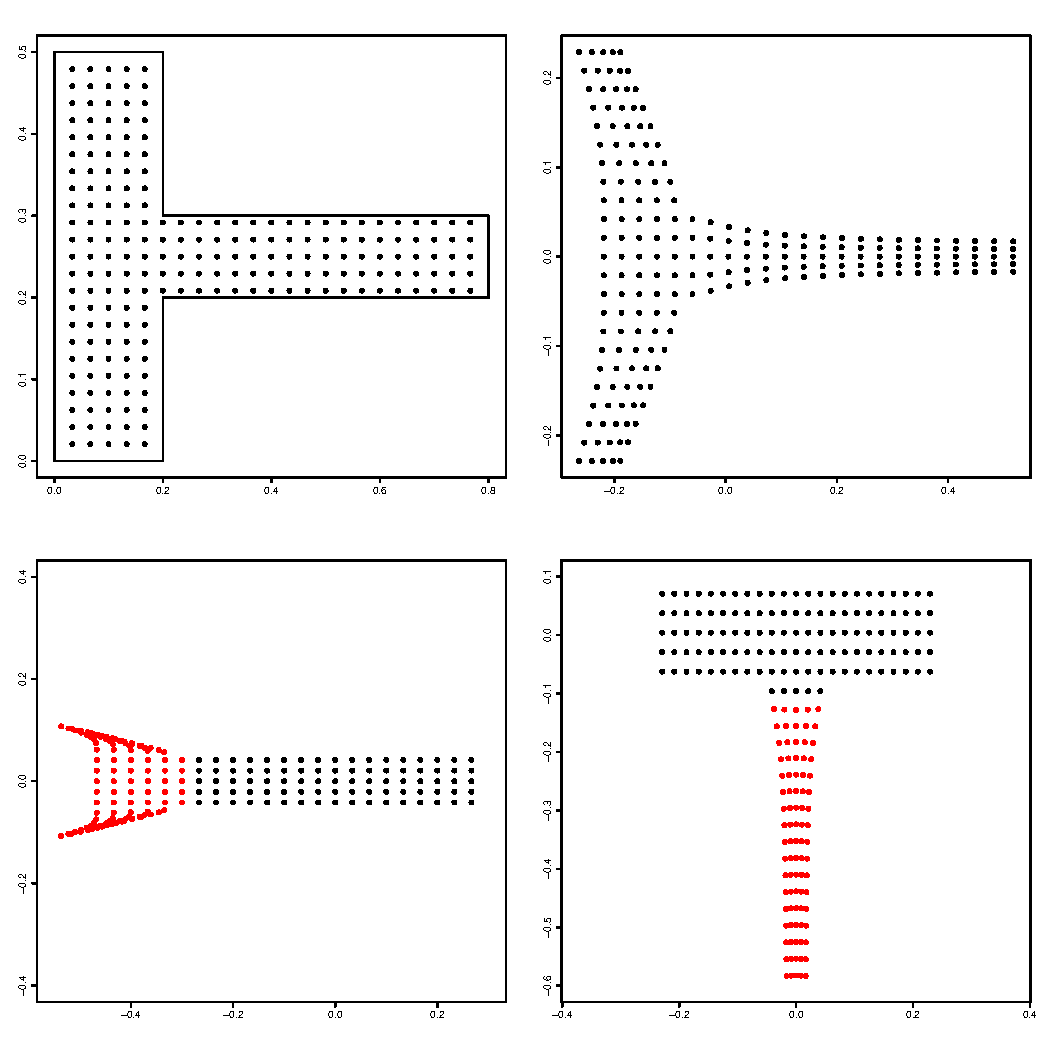
\includegraphics[width=3.5in]{figs/tshape.pdf} \\
\caption{Data generated inside a ``T'' shape (top left) is fed into MDS at once (top right.) When either the head or tail of the T is used for the original MDS configuration and the other points inserted, the shape produced is distorted.}
\label{tshape}
% generated using figs/gridtest.R
\end{figure}

Although the cases show in \fig{tshape} are somewhat pathological, looking at more reasonable situations still leads to wildly different results. In \fig{tshaperand} the black and green points make up the original MDS configuration; the five green points are chosen at random. The red points are then inserted. As can be seen in these four realisations, the shape of the MDS space is dependent on those points used to create the initial MDS configuration.

% showing the the grid is necessary using the T shape (random samples
\begin{figure}
\centering
% trim order l b r t
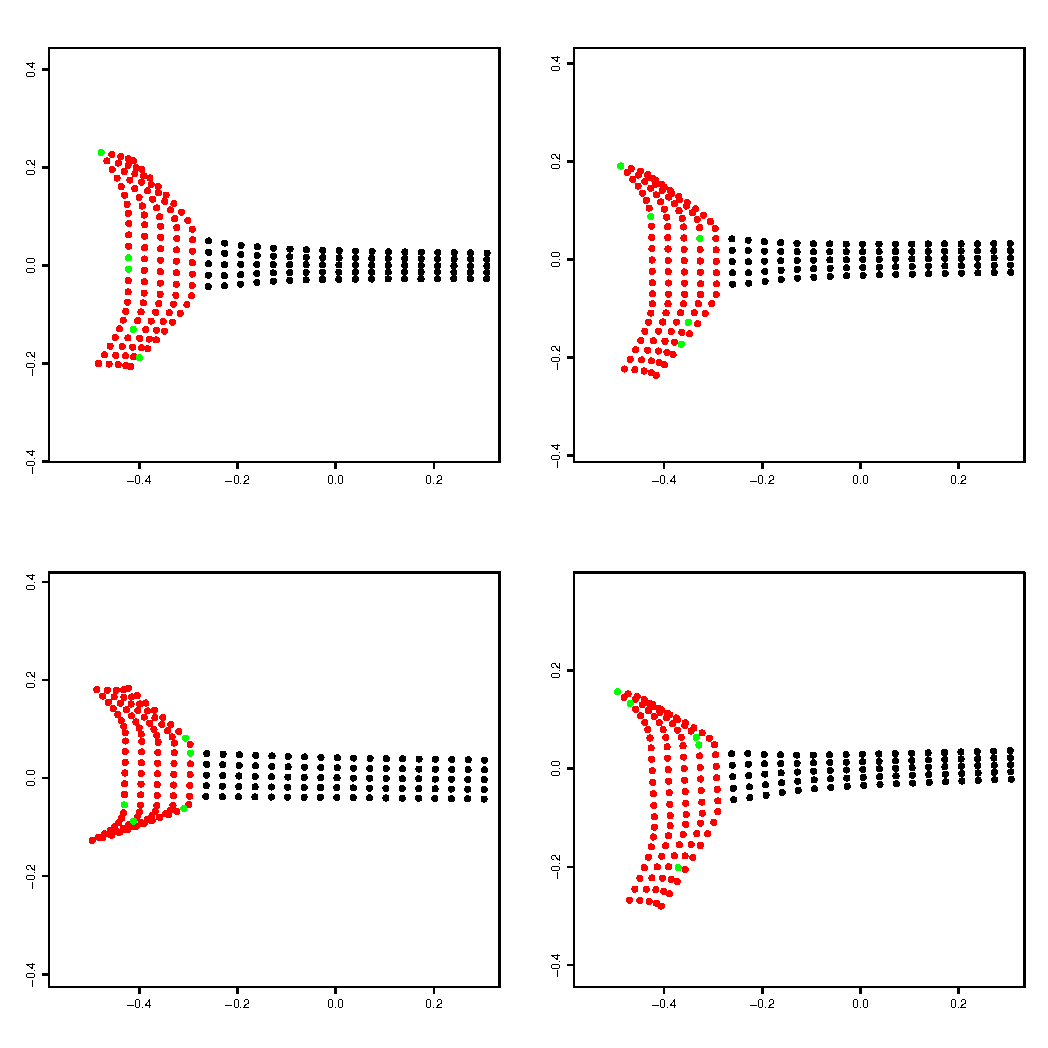
\includegraphics[width=3.5in]{figs/tshaperand.pdf} \\
\caption{Using the ``T'' shape in \fig{tshape}, the tail (black points) of the T was used with 5 randomly sampled (green) points in the head. The ``head'' (without the 5 green points) was then inserted into the MDS configuration (red.) As can be seen from these four realisations, the output varies greatly depending on the points sampled.}
\label{tshaperand}
% generated using figs/gridtest.R
\end{figure}

Hence, although there are the usual problems with predicting outside of one's dataset, the added problem of the instability of MDS insertion can only confound results further. (Again, this is mentioned at the end of Gower's paper.)

This problem can be rectified by using an appropriately spaced grid on the domain to calculate the eigen-decomposition, thus ensuring that the whole area is covered. The base MDS configuration is then stable, provided that the grid is fine enough to catch all the features in the boundary of the domain.

\subsubsection{Smoothness of mapping}

Following from this, it is important to make sure that the MDS space is smooth in the sense that a grid of smooth lines over the domain is mapped to a series of smooth lines without discontinuities or sudden changes in direction. Taking the evenly spaced grid in \fig{wt2-grid-orig}, first MDS is performed on a dense point set of size 1253, and then a less dense grid is inserted using the method of Gower. The grid produced under the insertion can be seen in \fig{wt2-grid-full}. Taking a sample of 250 points from the 1253, an MDS configuration was also found and the same grid inserted (see \fig{wt2-grid-samp}.) From this it is clear that those points mapped into the domain are smooth but in the sample case the features in the far right of the shape (the less pronounced peninsulae) are squashed down.

% grid to map
\begin{figure}
\centering
% trim order l b r t
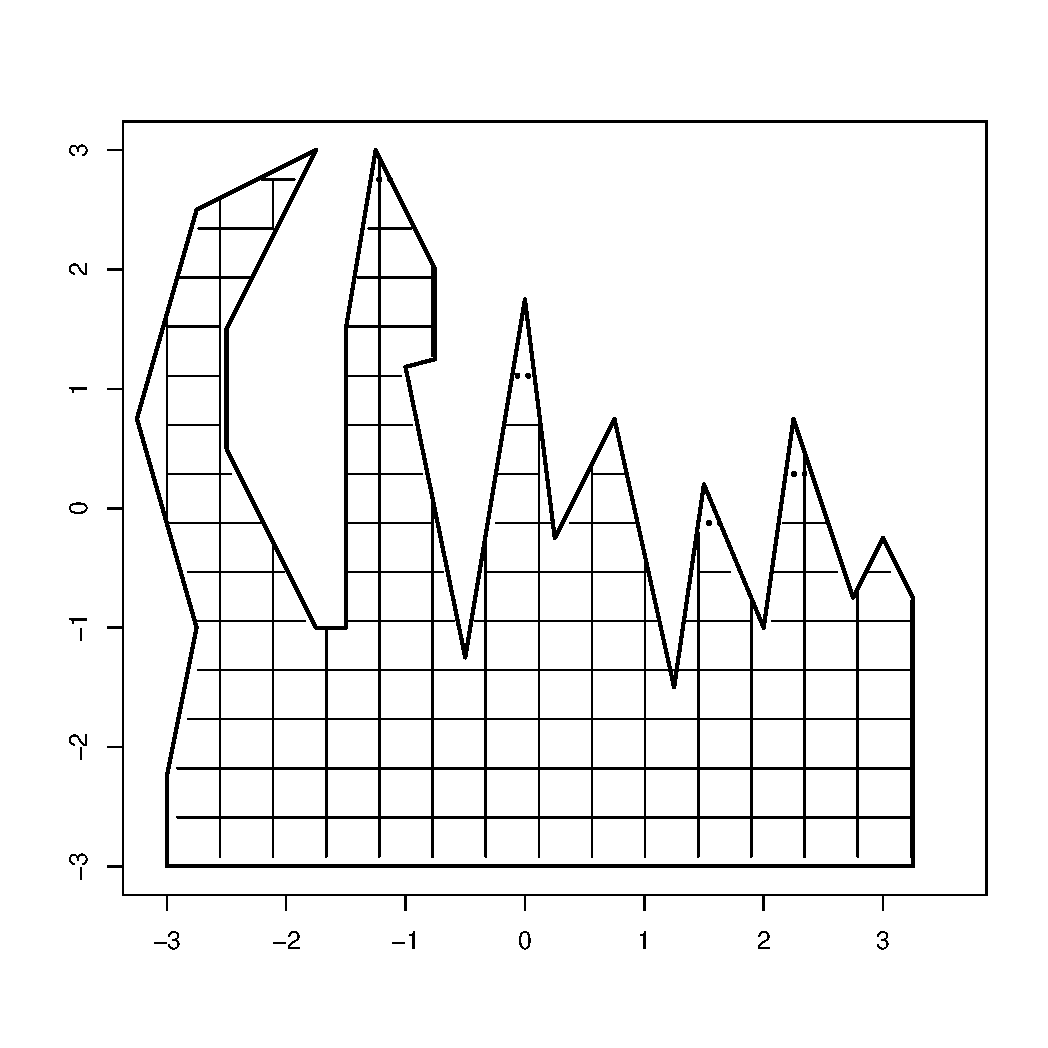
\includegraphics[width=4in]{figs/wt2-grid-orig.pdf} \\
\caption{The grid to be inserted into the MDS configuration.}
\label{wt2-grid-orig}
% generated using wt2-grid.R
\end{figure}

% mapped grid (full)
\begin{figure}
\centering
% trim order l b r t
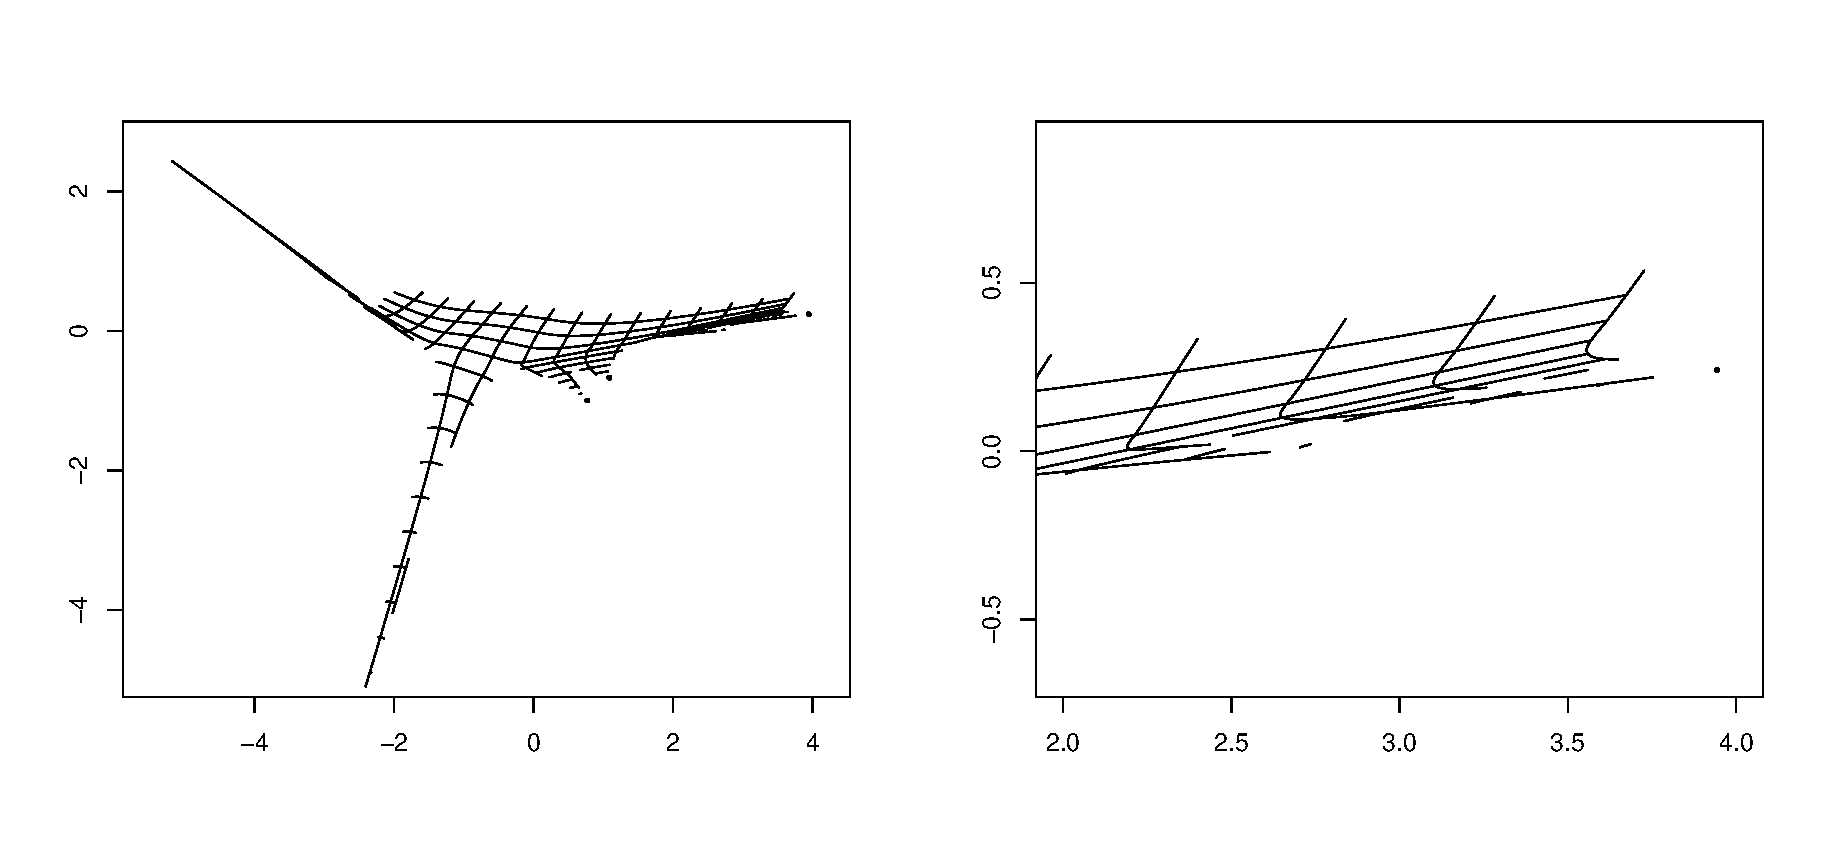
\includegraphics[width=5in]{figs/wt2-grid-full.pdf} \\
\caption{Inserted grid when 1253 points are used to create the initial MDS configuration. The right panel shows a zoom of the far right part of the configuration.}
\label{wt2-grid-full}
% generated using wt2-grid.R
\end{figure}

% mapped grid (samp)
\begin{figure}
\centering
% trim order l b r t
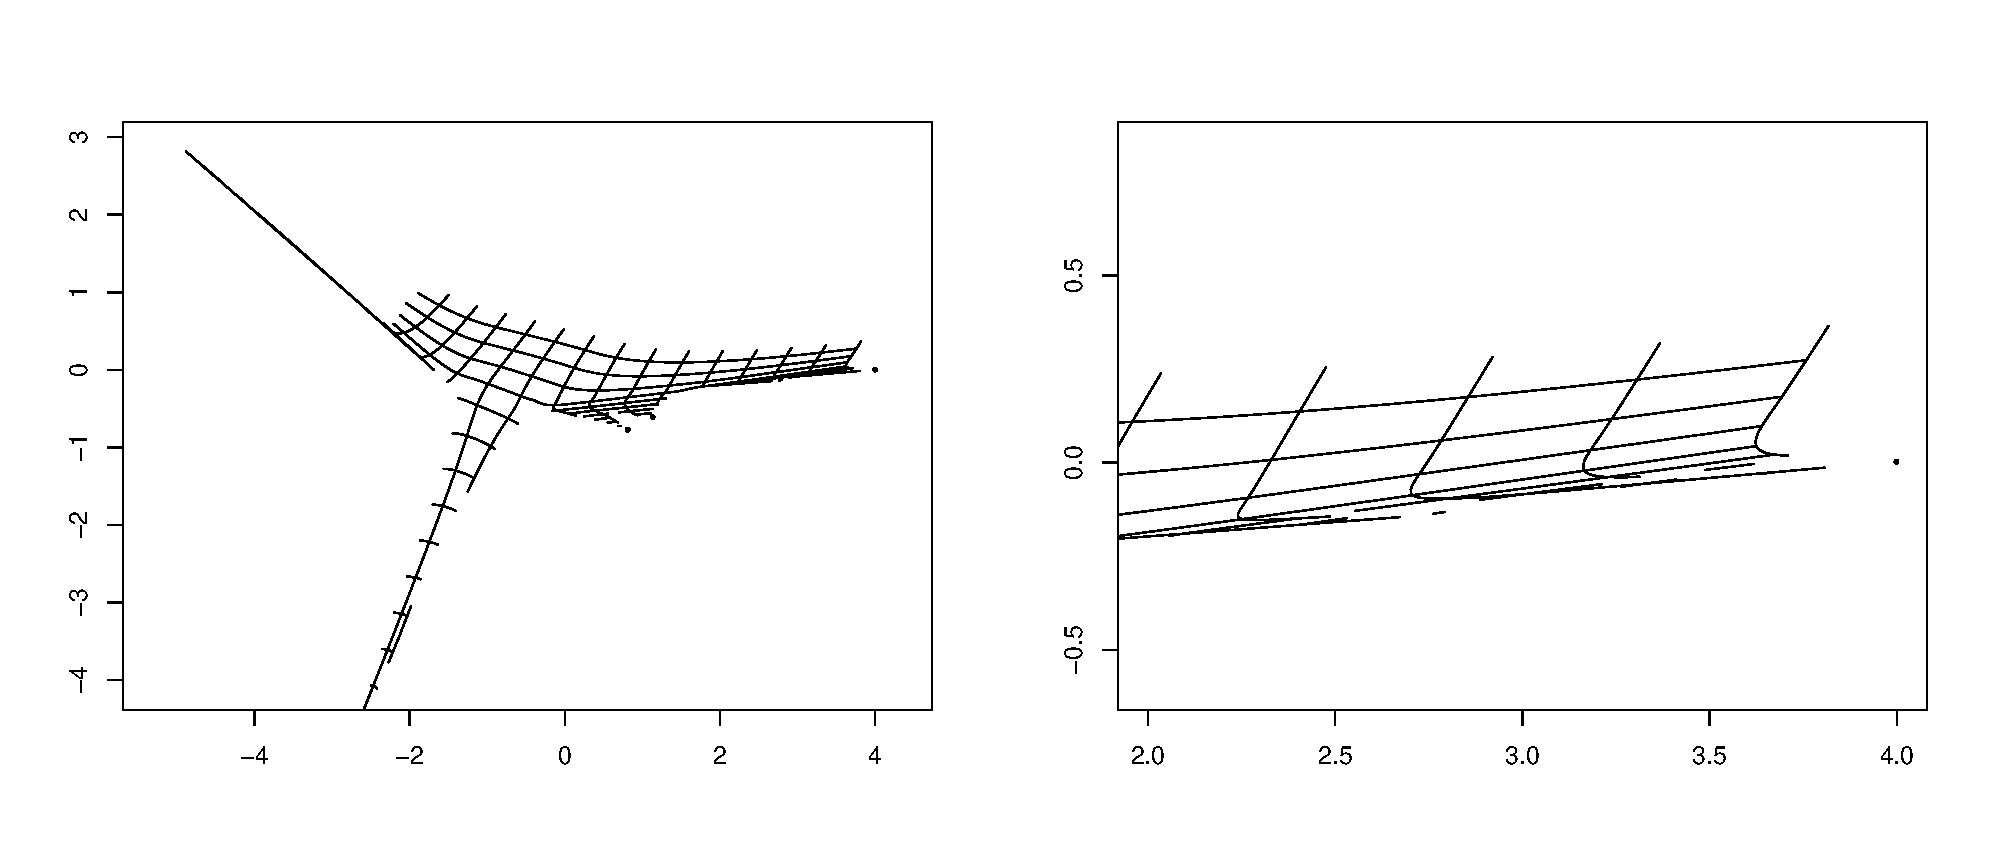
\includegraphics[width=5in]{figs/wt2-grid-samp.pdf} \\
\caption{Inserted grid when 250 randomly chosen points are used to create the initial MDS configuration. The right panel shows a zoom of the far right part of the configuration. Comparing this to that of \fig{wt2-grid-full}, one can see that the right side features have been squashed together.}
\label{wt2-grid-samp}
% generated using wt2-grid.R
\end{figure}

So, here we have seen that the mapping can be both reliable and also produces a smooth configuration of points provided that the initial MDS configuration covers the space in sufficient detail.


\section{Finding the within-area distances}

In order to perform multidimensional scaling the matrix of distances must be first found. In this case it makes sense to find the shortest distances between each pair of points where the path between the points lies entirely within the domain.

Given that there is no direct path within the domain (which can be considered as some polygon, $\Gamma$, say) between two points ($p_1$ and $p_2$, say), the algorithm proceeds as follows to create a path (ie. set of edges and vertices), $\mathcal{P}$:

\begin{enumerate}
\item (INIT) Start by drawing a line between $p_1$ and $p_2$ (\fig{wdia}, ($i$)). Start the path as the lines from $p_1$, $p_2$ to their first intersection with the boundary of $\Gamma$ ($p_1^1$, $p_2^1$, say.) Then form two paths between $p_1^1$ and $p_2^1$, composed of the intersection points and the vertices of $\Gamma$, one path in one direction $p_1^1$ to $p_2^1$ ($\mathcal{P}_1$), the other in the other direction, $p_2^1$ to $p_1^1$ ($\mathcal{P}_2$.) It is easy to see that $\{\mathcal{P}_1 \cup \mathcal{P}_2\} \setminus \{p_1^1, p_2^1\} = \Gamma$ (\fig{wdia}, ($ii$).) Finding the length of $\mathcal{P}_1$ and $\mathcal{P}_2$ and choosing the shorter ($\mathcal{P^*}$), the initial path is formed as $\mathcal{P}=(p_1,p_1^1,\mathcal{P}^*,p_2^1,p_2)$ (\fig{wdia}, ($iii$).) 

\item (DELETE) Given a triple of vertices, $(v_i, v_{i+1}, v_{i+2}) \in \mathcal{P}$ , if the line between $v_i$ and $v_{i+2}$ is shorter than the path $(v_i, v_{i+1}, v_{i+2})$ and the line between $v_i$ and $v_{i+2}$ lies inside $\Gamma$ then delete $v_{i+1}$ (\fig{wdia}, ($iv$) and ($vi$).) The entire path is iterated over deleting all superfluous vertices until there are no changes in successive runs. For example in \fig{wdia}, ($iii$) $v_2$ is deleted from $\mathcal{P}$ because the path straight between $v_1$ and $v_3$ is shorter. 

\item (ALTER) Given a triple of vertices $(v_i, v_{i+1}, v_{i+2})$, if the path $(v_i, v^1_1, \mathcal{P}_I, v^1_j, v_{i+2})$ is shorter than the path $(v_i, v_{i+1}, v_{i+2})$ then replace $v_{i+1}$ with $v^1_1, \mathcal{P}_I, v^1_j$ (\fig{wdia}, ($v$)). The candidate replacement path can be thought of as the result of running INIT with $p_1$ and $p_2$ replaced with $v_i$ and $v_{i+2}$ and then using DELETE to remove superfluous vertices. Here $v^1_1$ and $v^1_j$ are equivalent to $p_1^1$ and $p_2^1$ in INIT and $\mathcal{P}_I$ to $\mathcal{P}^*$ (but after having had DELETE remove the unnecessary vertices.) For example in \fig{wdia} ($iv$), the path $(v_1, v_2, v_3)$ is longer than the path $(v_1, v^1_1, v^1_2, v^1_3, v_3)$ so the former is replaced with the latter in $\mathcal{P}$.

\item (ITER) We then iterate between the DELETE and ALTER steps until there has been no change from one run to the next (ie. convergence) or there have been too many iterations (\fig{wdia}, ($vi$).)
\end{enumerate}

% diagram for finding the shortest path in W
\begin{sidewaysfigure}
\centering
% trim order l b r t
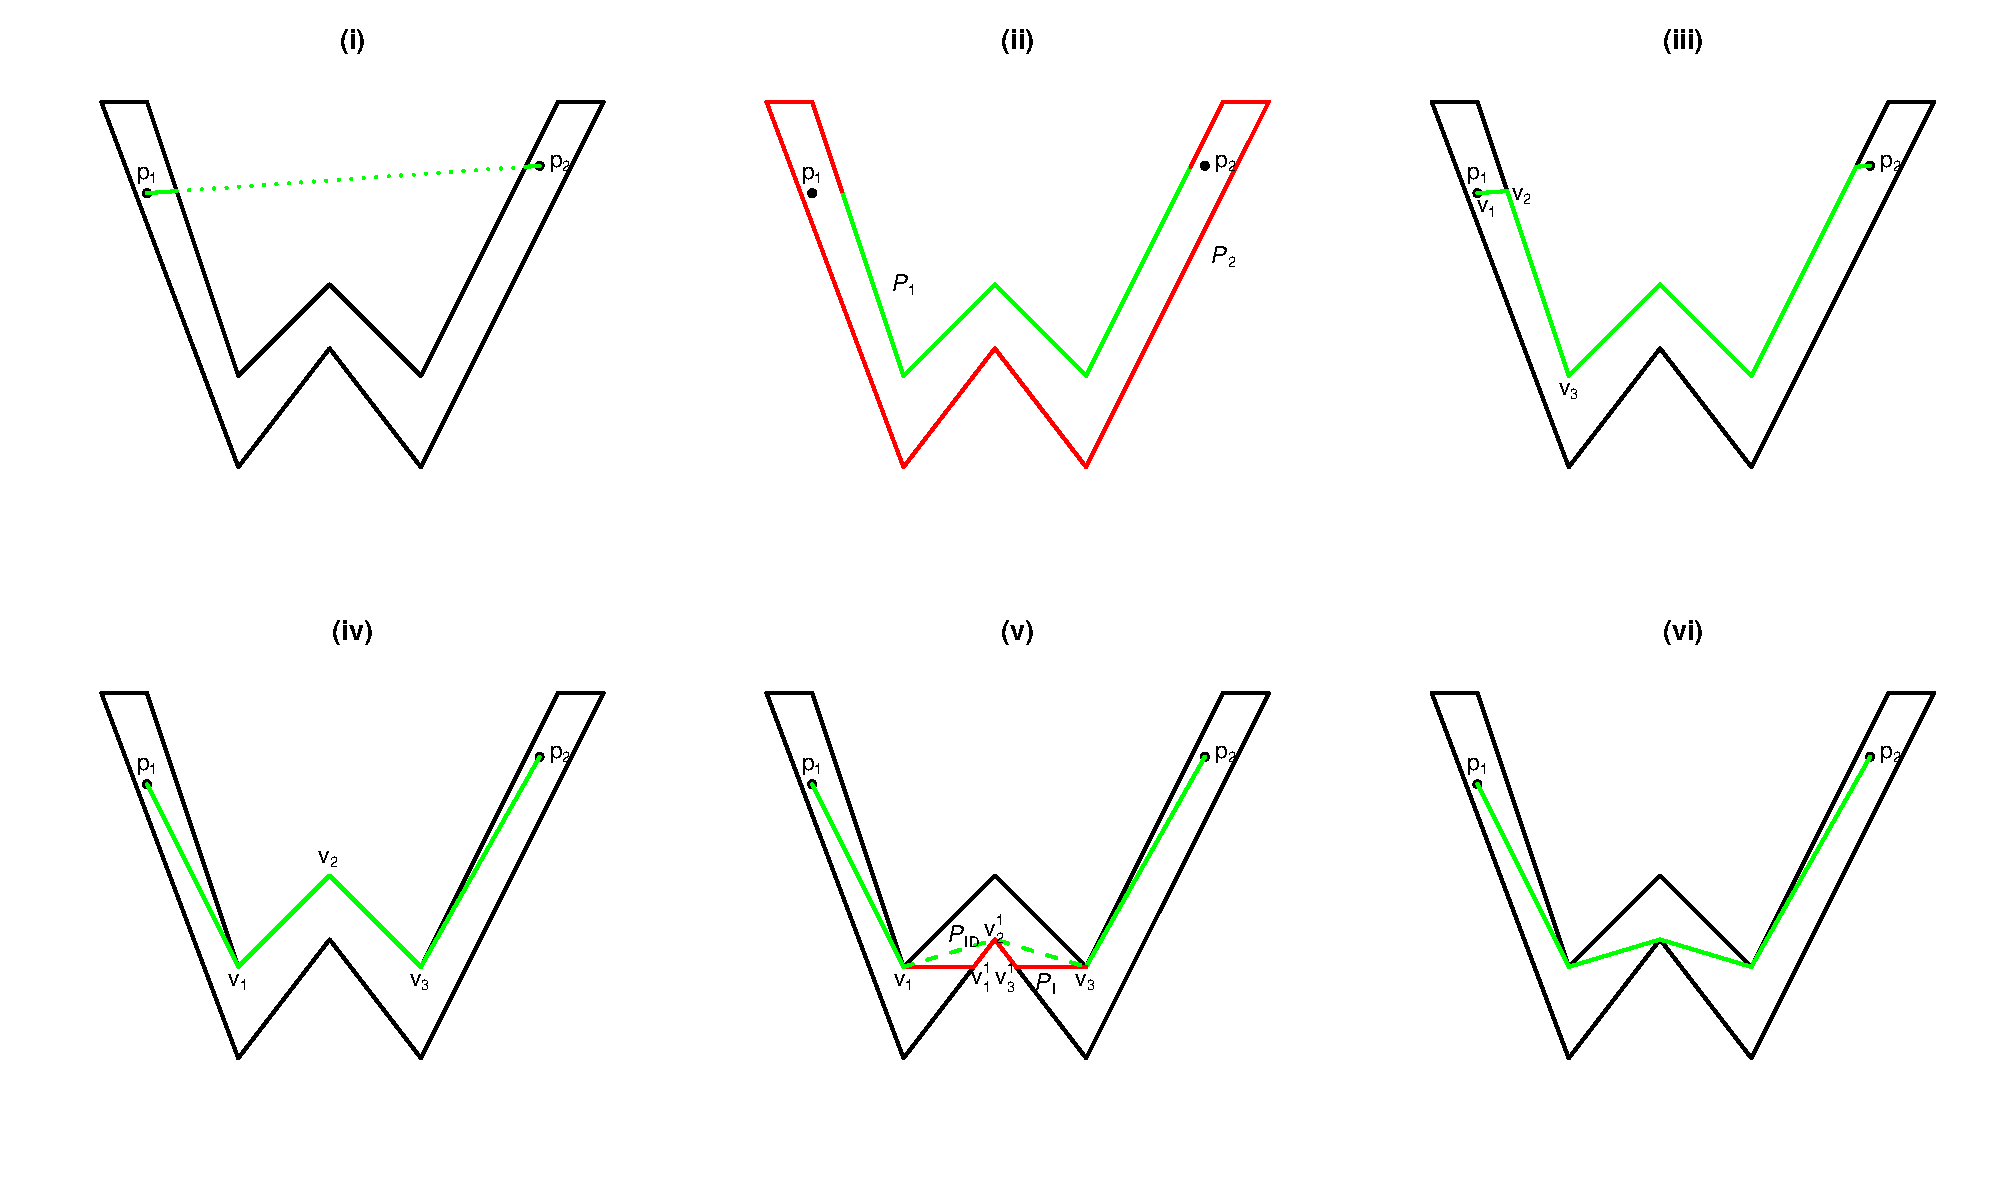
\includegraphics[trim=0in 0.5in 0in 0.25in, width=9.5in]{figs/wdia.pdf} \\
\caption{The green lines in ($i$) to ($vi$) show the path as the algorithm progresses from initial state to final, shortest path (bottom right.) }
\label{wdia}
% generate /phd-smoothing/mds-writeup/figs/distanceexplanation.R
\end{sidewaysfigure}

Of course, if there is a direct path between $p_1$ and $p_2$ then the Euclidean distance between the points can be used.

\section{Multidimensional scaling for smoothing over complex domains}

Taking a cue from \cite{soap} simulations were conducted on the so-called modified Ramsay horseshoe and another domain supposed to mimic the shape of a coastline. Results are compared using the mean squared error (MSE) criterion and their estimated degrees of freedom (EDF.)

The mean squared error is defined (as in \cite{simonbook} p. 131) as:

\begin{equation}
\text{MSE}(\hat{f}) = \frac{1}{P} \sum_{j=1}^P (\hat{f}(x_j) - z_j)^2,
\end{equation}
the mean difference between the model ($\hat{f}$) evaluated at the prediction points ($\{x_j : j=1 \dots P\}$) and the true value of the function ($\{z_j : j=1 \dots P\}$.) This gives the MSE per model, since here many realisations are run, the mean of these over all simulations is taken and the standard error is calculated.

The estimated degrees of freedom of a model gives an idea of the complexity of the spline that was fit to the data, the higher the EDF, the more basis functions were used and  the more complex the model.  Since the models used here are penalised, it is the penalty term that controls the overall ``wigglyness'' of the spline and hence the EDF. Although the basis dimension is set in the model this is just an upper bound, the smoothing penalty suppresses parts of the model. Therefore basis dimension is not a major concern provided that it is not set too low (\cite{simonbook}, p. 161.) 


\subsection{Modified horseshoe}

The domain in \fig{leakage} is known as the modified Ramsay horseshoe. It is based on the horseshoe-like shape used in \cite{ramsay} and clearly illustrates the problem of leakage. It differs from the figure in \cite{ramsay} in that a slight curvature in the function along the major axis has been added such that the gradient is not perpendicular to the boundary. This curvature was added in \cite{soap}  in order to avoid the horseshoe function lying in the nullspace of the soap film's penalty, making the problem too easy for a soap film smoother.

For the modified horseshoe, 100 replications of samples of 250 points with normal errors (at 3 levels: 0.1, 1 and 10) were run. From these samples, three models were fitted to the data and predictions over 718 points (including the sample locations) and the mean squared error was calculated between the model prediction and the true function value for the horseshoe. The three models fitted were as follows using the \textsf{R} packages \texttt{mgcv} and \texttt{soap}:

\begin{enumerate}
\item \emph{Thin plate spline}: bivariate thin plate spline with basis size 100.
\item \emph{Soap film smoother}: 32 knots evenly spread over a grid over the domain, cyclic spline on the boundary was of basis size 39.
\item \emph{MDS}: Used a thin plate spline of basis dimension 100. The initial MDS grid was 20 points wide by 10 points tall.
\end{enumerate} 

In all cases smoothing parameter estimation was performed using GCV.

Note that due to time and computational restrictions, the boundary was reduced from the 160 vertex polygon in the \texttt{fs.boundary()} function in \texttt{soap} to a 21 vertex polygon by only using every 8$^\text{th}$ vertex.

\begin{table}[ht]
\centering
\begin{tabular}{c c c c}
 & & MSE & \\ 
$\sigma$ & MDS & Soap film & Thin plate\\ 
\hline
0.1  & 0.0032 (3$\cross10^{-5}$) & 0.0022 (3$\cross10^{-5}$) & 0.0402 (0.0008) \\ 
1  & 0.0436 (0.0015) & 0.0482 (0.0014) & 0.2306 (0.0024) \\ 
10  & 2.0652 (0.1215) & 3.0702 (0.2382) & 3.3713 (0.1133) \\ 
\end{tabular}
\begin{tabular}{c  c c c }
&  & EDF & \\ 
$\sigma$ & MDS & Soap film & Thin plate\\ 
\hline
0.1 & 47.613 (0.3497) & 39.164 (0.26) & 92.5996 (0.1020)\\ 
1  & 8.3828 (0.3452) & 11.868 (0.4010) & 46.607 (0.4238)\\ 
10 & 5.0577 (0.3324) & 5.5863 (0.2876) & 5.9786 (0.2511)\\ 
\end{tabular}
\caption{Mean MSE and estimated degrees of freedom (EDF) for the three models fitted to the modified Ramsay horseshoe function with standard errors (in brackets) over 200 realisations.}
\label{ramsayresultstable}
\end{table}

A typical realisation from the models can be seen from \fig{ramsay-fit-1}, where $\sigma=1$ with a sample size of 250. Both the soap film smoother and MDS have respected the boundary and, even with relatively high noise and low sample size, they reproduce the true function fairly well. The thin plate regression spline, on the other hand, shows leakage as expected. This is reflected in table \ref{ramsayresultstable} where we see that the soap film smoother and MDS perform significantly better in terms of mean squared error. It also seems that the MDS performs better than the soap film when there is a high degree of noise in the data.

The EDFs in table \ref{ramsayresultstable} show that the MDS approach always gives a less complex model than using a thin plate spline, and for the two higher error situations, has a lower EDF than the soap film. Given that this is coupled with a lower MSE, it seems that the MDS approach yields both a more accurate and less complex model for the Ramsay horseshoe when there is high noise.

% Ramsay fit with error=1 
\begin{figure}
\centering
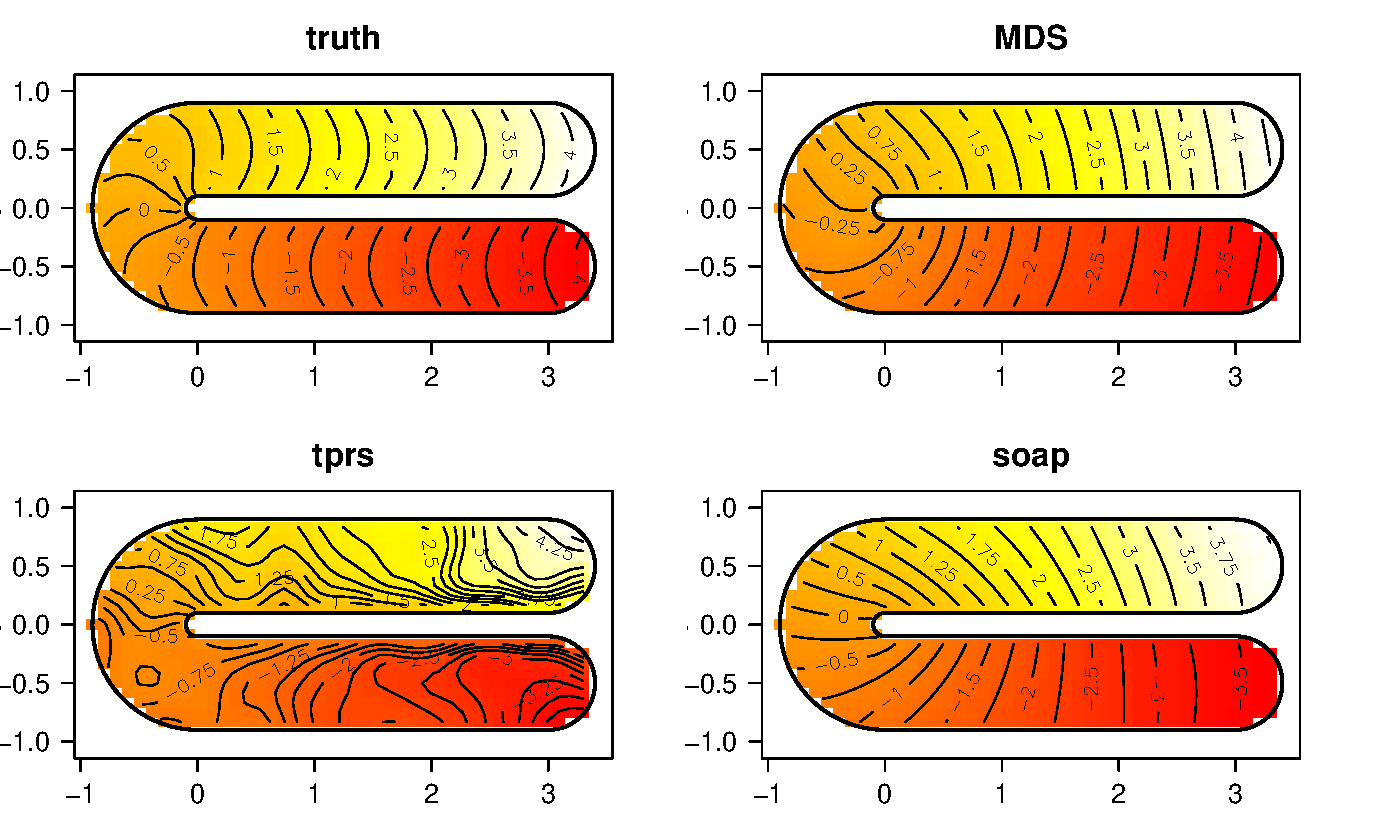
\includegraphics[width=6in]{figs/ramsay-fit-1.pdf} \\
\caption{Top left: truth for the (modified) Ramsay horseshoe. Others: a typical realisation of fits from the three models when 250 points are sampled with noise set to $\sigma=1$.}
\label{ramsay-fit-1}
% generated (roughly) using ramsay-smooth-test.R
\end{figure}

\subsection{Peninsulae domain}

The Ramsay horseshoe is, in a sense, easy domain to smooth over since it is obvious what the transformation should be doing. For this reason a more complex and more realistic domain would provide more insights into the efficacy of the method. The domain shown in \fig{wt2-truth} is an approximation to a coastline with a strong trend along both peninsulae (in a manner similar to that of the horseshoe) but with the added complication of a further peak in the lower right corner.

Again, 200 realisations from the domain shown in \fig{wt2-truth} were used with Normal errors at 3 levels of $\sigma$ (0.05, 0.5 and 5.) Mean squared error over 1253 prediction points (including those points in the sample) was calculated from fitting models with 250 samples. The models fitted were:

% wt2 truth 
\begin{figure}
\centering
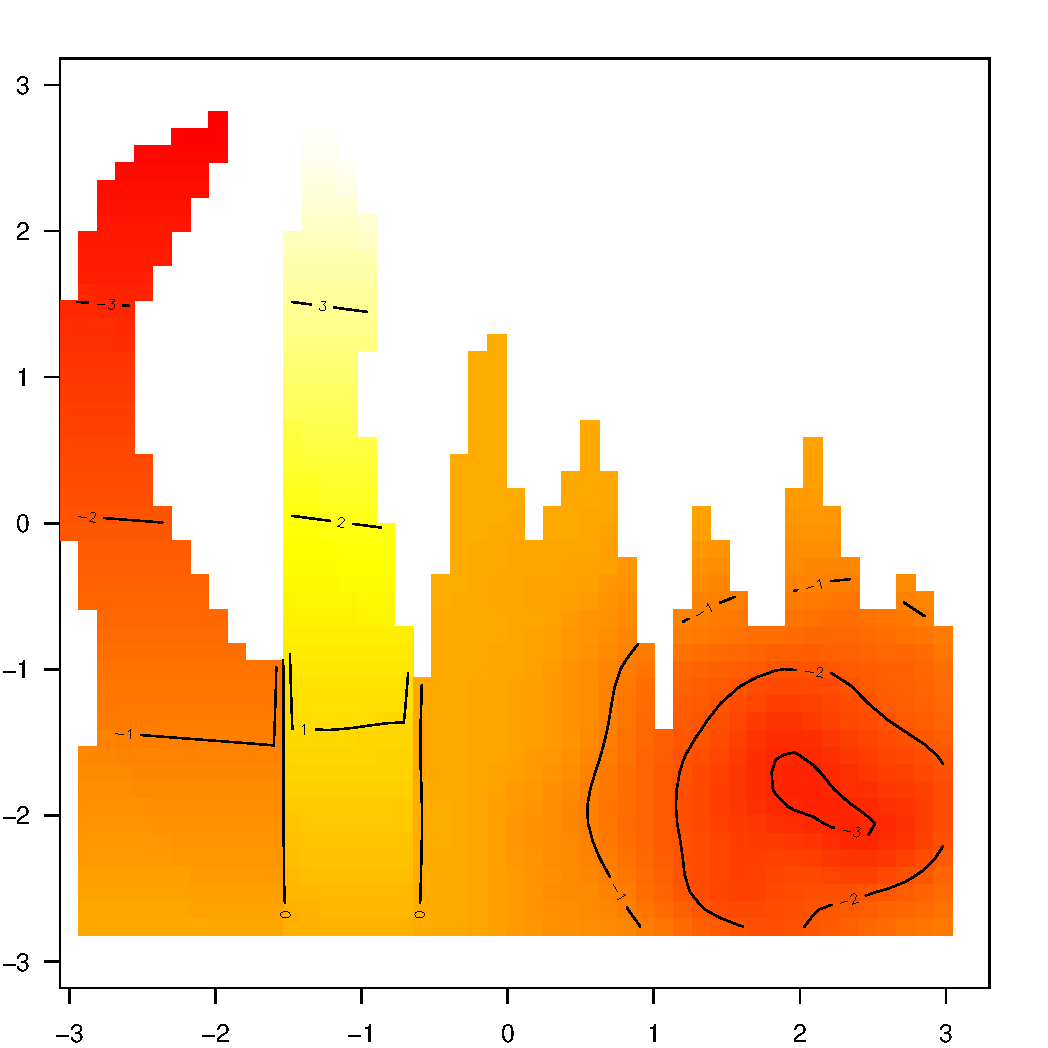
\includegraphics[width=3in]{figs/wt2-truth.pdf} \\
\caption{True function for the domain with multiple peninsulae.}
\label{wt2-truth}
% generated (roughly) using wt2-smooth-test.R
\end{figure}

\begin{enumerate}
\item \emph{Thin plate spline}: bivariate thin plate spline with basis size 100. 
\item \emph{Soap film smoother}: cyclic spline on boundary of basis size 60, 109 internal knots evenly spaced over the domain on a grid.
\item \emph{MDS}: after transform a bivariate thin plate spline with basis size 100 was fit. The initial MDS grid was 74 points square.
\item \emph{MDS with tensor product}: tensor product of two thin plate splines, each of basis dimension 12. The initial MDS grid was 74 points square.
\end{enumerate} 

In all cases smoothing parameter estimation was performed using GCV.

Looking at a typical realisation in \fig{wt2-fit-0.5}, we see that soap (bottom right panel) does very well, as can be expected, and the thin plate spline (\fig{wt2-fit-0.5}, bottom left panel) fit shows leakage (again, as can be expected.) 

The final model, above, was chosen after it appeared that the MDS with a bivariate thin plate spline did not adequately model the peak in the right corner of the domain (\fig{wt2-fit-0.5}, top left panel.) After using a tensor product of thin plate splines a better fit to the right peak was found (\fig{wt2-fit-0.5}, top right panel), although this is not reflected particularly well in terms of mean squared error (see table \ref{wt2resultstable}.) The visual improvement in fit can be explained by thin plate splines in two dimensions being an isotropic smooth and since space has not been transformed in a uniform way in both dimensions.

Table \ref{wt2resultstable} shows that when there is low error, both the soap film and thin plate splines outperform the MDS approach, but once the errors are increased the MDS does much better. The MDS approach also benefits from having a smaller EDF than all the other approaches in all of the noise scenarios, the tensor MDS doing better at lower noise levels. This is encouraging and shows that perhaps there is a place for this technique alongside the soap film smoother if the method can be improved for low noise situations.

\begin{table}[ht]
\centering
\begin{tabular}{c c c c c}
 &  & MSE  & &\\ 
$\sigma$ & MDS & MDS (tensor) & Soap film & Thin plate\\ 
\hline
0.05  & 0.0948 (0.00084) & 0.0603 (0.00352) & 0.0237 (0.00039) &0.0504 (0.00039) \\ 
0.5  & 0.1426 (0.00078) & 0.1106 (0.00133) & 0.1013 (0.02151) &0.1123 (0.02151) \\ 
5  & 0.9179 (0.02644) & 1.2481 (0.04159) & 1.1987 (0.04111) &1.3865 (0.04111)\\ 
\end{tabular}
\begin{tabular}{c c c c c}
 &  & EDF  & &\\ 
$\sigma$ & MDS & MDS (tensor) & Soap film & Thin plate\\ 
\hline
0.05 &72.262 (0.89606) & 78.2691 (0.679) & 94.5187 (0.78697) & 86.9415 (0.78697)\\ 
0.5 &40.7981 (0.46687) & 50.5025 (0.36223) & 45.2341 (0.74063) & 58.418 (0.74063)\\ 
5  &6.8274 (0.36097) & 8.577 (0.3649) & 11.5419 (0.83982) & 11.9407 (0.83982)\\ 
\end{tabular}

\caption{Mean MSE and EDF for the four models fitted to the peninsula domain with standard errors (in brackets) over 200 realisations.}
\label{wt2resultstable}
\end{table}




% wt2 fit with error=0.5
\begin{figure}
\centering
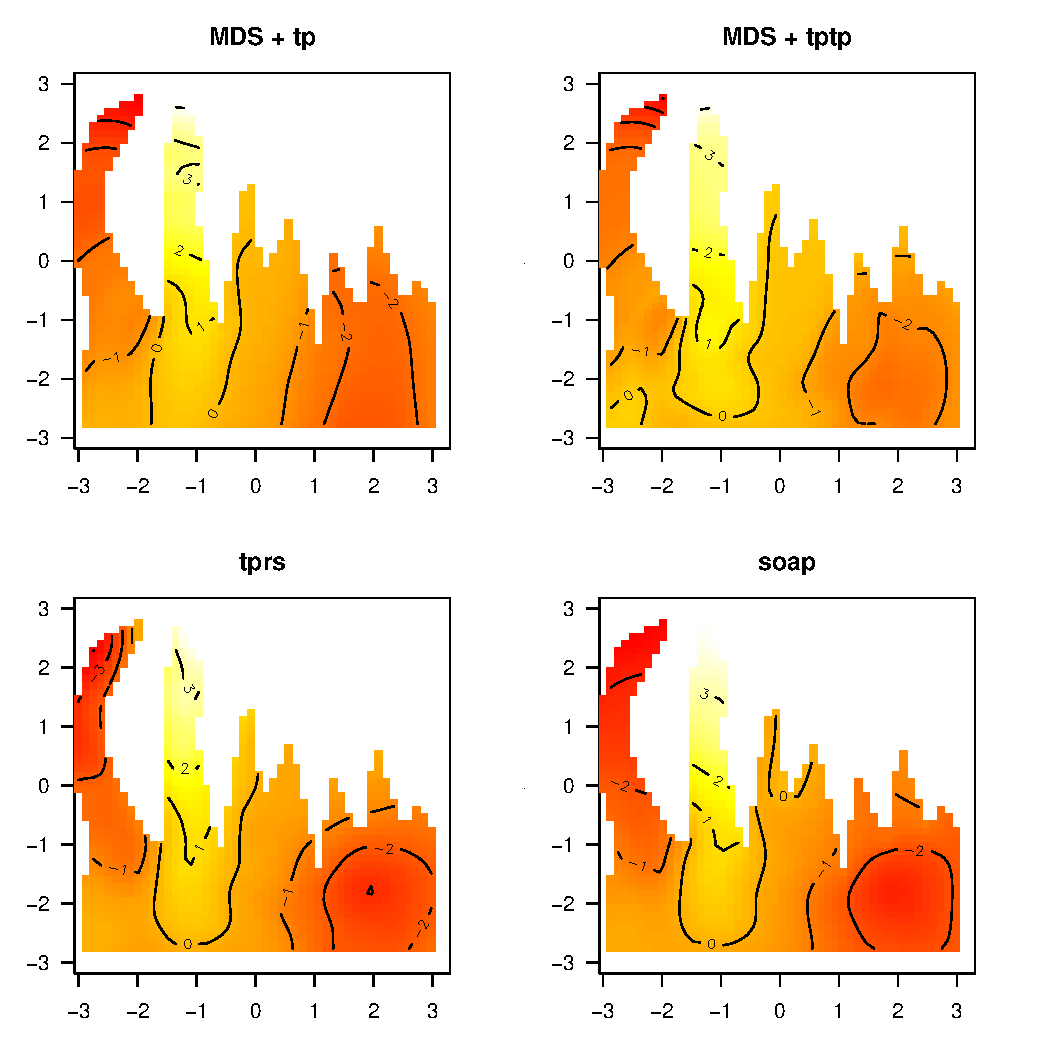
\includegraphics[width=6in]{figs/wt2-fit-05.pdf} \\
\caption{A typical realisation of fits from the multiple peninsulae domain when $\sigma$ is set to 0.5.}
\label{wt2-fit-0.5}
% generated (roughly) using wt2-smooth-test.R
\end{figure}



\section{Conclusions}

Although these results are encouraging, the inability of the smooth to capture all the features in the right side of the domain when using an isotropic smoother is disappointing. Proposed further work is to follow the lead from \cite{wood2000}, which shows that given some transform of a variable, $y$ say, such that $y_i^\prime=y_i/k$, then $f(x,y^\prime k)$ will give the same fit as $f(x,y)$ (ie. the fit will be the same under the new coordinates) but the penalty will change to:
\begin{equation}
\int\int_\Omega \Big( \frac{\partial^2 f}{\partial x^2} \Big) + 2k\Big( \frac{\partial^2 f}{\partial x \partial y} \Big) + k^3\Big( \frac{\partial^2 f}{\partial y^2} \Big) \text{d}x \text{d}y,
\label{adjustedintegral}
\end{equation}
from:
\begin{equation*}
\int\int_\Omega \Big( \frac{\partial^2 f}{\partial x^2} \Big) + 2\Big( \frac{\partial^2 f}{\partial x \partial y} \Big) + \Big( \frac{\partial^2 f}{\partial y^2} \Big) \text{d}x \text{d}y.
\end{equation*}
In the case of the MDS, the integral would need to be split over a grid such that each cell captured the distortion in space over the area of the cell. Mathematically, $\Omega$ would be split into a subsets, $\omega_i$ (where $\bigcup_{\forall j} \omega_j = \Omega$) and (\ref{adjustedintegral}) becomes:
\begin{equation}
\sum_{\forall j} \int\int_{\omega_j} l_j^3 \Big( \frac{\partial^2 f}{\partial x^2} \Big) + 2k_jl_j\Big( \frac{\partial^2 f}{\partial x \partial y} \Big) + k_j^3\Big( \frac{\partial^2 f}{\partial y^2} \Big) \text{d}x \text{d}y,
\end{equation}
where $k_j$ is the scaling in the $y$ direction and $l_j$ is the scaling in the $x$ direction for the $j^{\text{th}}$ cell. We assume here that $f(x,y)$ is ``nice''.

Using this penalty may allow for the distortions in space to be taken account of and therefore get around the problem of the details being smoothed over, as seen above. It will be easiest to first build this using a tensor product of $P$-splines to test its utility (since their penalty is discrete) and then move on to the thin plate spline penalty.

In order to make this MDS approach competitive with \texttt{soap} (assuming that the above distortion adjustment is successful) a speed-up in the computation of the within-area distances must be achieved. At the moment this is the major bottleneck in the calculation since model fitting consists only of fitting a thin plate spline. 


\begin{table}[ht]
\centering
\begin{tabular}{c || c c c}
 & MDS & Soap film & Thin plate\\ 
\hline
Fit & 3.39225 & 10.87688 & 0.61492\\
Prediction & 4.80357 & 8.87535 & 0.10845\\
\end{tabular}
\label{ramsaytime}
\caption{Average time (in seconds) to fit a realisation of the modified Ramsay horseshoe for the three models considered above. Times are averaged over 100 realisations and were found using the elapsed time provided by \textsf{R}'s built-in \texttt{system.time} function.}
\end{table}


\begin{table}[ht]
\centering
\begin{tabular}{c || c c c c}
 & MDS & MDS (tensor) & Soap film & Thin plate\\ 
\hline
Fit & 84.85242 & 85.35168 & 36.24865 & 0.51721\\
Prediction & 155.4004 & 155.2419 & 44.22065 & 0.20994 \\
\end{tabular}
\label{wt2time}
\caption{Average time (in seconds) to fit a realisation of the peninsula domain for the four models considered above. Times are averaged over 100 realisations and were found using the elapsed time provided by \textsf{R}'s built-in \texttt{system.time} function.}
\end{table}


Speed-ups can be achieved by minimizing the number of calculations for within-area distance that are needed. In \cite{landmark} a method to calculate MDS coordinates using a sparse grid of landmark points is suggested; although the authors are sceptical about how this will perform with non-Euclidean distances. There is clearly some work here in finding some minimal set of landmark points for the within-area distance metric obtained from the above algorithm.

The calculation of within-area distances could be linked into a ``landmark''-type process by calculating the within-area distances between a set of points in a sparse grid, then saving those paths. The distances between desired points can then be found by modifying the path with the end points nearest to those of the desired points.


\bibliographystyle{chicago}
\bibliography{mds-refs}

\end{document}
